\documentclass[12pt, a4paper]{article}

\usepackage[T1, T2A]{fontenc}
\usepackage[utf8]{inputenc}
\usepackage[russian]{babel}
\usepackage{indentfirst}
\usepackage{graphicx}
\usepackage{xcolor}
\usepackage{titlesec}
\usepackage{wrapfig}

\graphicspath{ {./images/} }

\setlength{\unitlength}{1cm}

\titleformat{\section}[block]
{\Large\normalfont\bfseries\filcenter}
{}{1em}{}

\titleformat{\subsection}[hang]
{\large\normalfont\bfseries\filcenter}
{}{1em}{}

\titleformat{\subsubsection}[block]
{\normalsize\normalfont\bfseries\filright}
{}{1em}{}

\title{\textbf{Изучение экспериментальных погрешностей на
примере физического маятника}}
\author{Солодилов Михаил Б01-307}
\date{9.10.2023}

\begin{document}

\maketitle
\tableofcontents

\newpage

\section{Аннотация}

\textbf{Цель работы:}
\begin{enumerate}
    \item на примере измерения периода свободных колебаний физического
    маятника познакомиться с систематическими и случайными погрешностями, 
    прямыми и косвенными измерениями;
    \item  проверить справедливость формулы для периода колебаний физического
    маятника и определить значение ускорения свободного падения;
    \item убедиться в справедливости теоремы Гюйгенса об обратимости
    точек опоры и центра качания маятника;
    \item оценить погрешность прямых и косвенных измерений и конечного
    результата.
\end{enumerate}

\textbf{В работе используются:} металлический стержень с опорной призмой;
дополнительный груз; закреплённая на стене консоль; подставка с острой гранью
для определения цента масс маятника; счётчик колебаний электронный; линейки
металлические различной длины; штангенциркуль; электронные весы.

\newpage

\section{Теоретические сведения}

\begin{wrapfigure}{r}{0.46\textwidth}
    \centering
    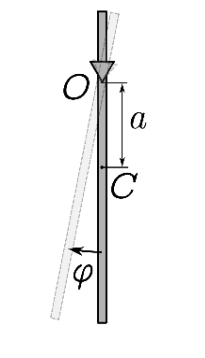
\includegraphics[width = 0.25\textwidth]{Figure 1}
    \caption{стержень как физический маятник}
\end{wrapfigure}

\textit{Физическим маятником} называют \textit{твёрдое тело}, способное
совершать колебания в вертикальной плоскости, будучи подвешено за одну из
своих точек в поле тяжести. Основное отличие физического маятника от
математического в том, что маятник не является точечным объектом, а
представляет собой совокупность жёстко связанных точечных масс. В данной
работе в качестве такого маятника используется тонкий однородный металлический
стержень, подвешиваемый в некоторой точке с помощью небольшой опорной призмы
(см. рис. 1). Острое ребро призмы, опирающееся на подставку, задаёт 
\textit{ось качания} (или вращения) маятника.

Момент инерции $J$ однородного стержня длиной $l$, массой $m$ относительно
его центра масс выражается следующим образом:

\[J_c = \frac{ml^2}{12}.\]

А момент инерции стержня, подвешенного на расстоянии $a$ от центра масс,
может быть вычислен по теореме \textit{Гюйгенса–Штейнера}:

\begin{equation}
    J = \frac{ml^2}{12} + ma^2.
\end{equation}
В частности, если подвесить стержень за один из концов, то
$a = \frac{l}{2}$ и $J = \frac{ml^2}{3} \text{см}$.

\subsubsection*{Стержень как физический маятник}

Вернёмся к рассмотрению колебаний физического маятника —
стержня, подвешенного в поле тяжести (Рис. 1). Маятник подвешен в
точке $O$ на расстоянии $a$ до центра масс $C$. При отклонении стержня от
вертикального положения равновесия на угол $\phi$ возникает момент силы
тяжести, стремящийся вернуть стержень в исходное положение. Плечо этой
силы, приложенной к точке $C$, относительно оси подвеса $O$ равно
$a\sin{\phi}$, поэтому при небольших углах отклонения $\phi \ll 1 $
возвращающий момент равен:

\[M = -mga\sin{\phi} \approx -mga\phi\]

Таким образом, на маятник действует возвращающий момент
\newline
сил, пропорциональный
величине его отклонения от равновесия. Отсюда можно сделать вывод, что при
малых \textit{амплитудах} отклонения движение свободного физического маятника
будет иметь характер \textit{гармонических колебаний}, аналогично колебаниям
груза на пружине или математического маятника. 

Чтобы получить формулу периода колебаний физического маятника,
воспользуемся аналогией с пружинным маятником, период колебаний которого
равен, как известно, $T = 2\pi\sqrt{\frac{m}{k}}$. Здесь роль массы $m$,
как мы уже обсудили, играет момент инерции тела $J$, а роль коэффициента
жёсткости пружины $k$ — коэффициент пропорциональности между моментом силы и
величиной отклонения $mga$. Таким образом, приходим к следующей общей формуле
для периода колебаний произвольного физического маятника:

\begin{equation}
    T = 2\pi\sqrt{\frac{J}{mga}}
\end{equation}

А для стержня длиной $l$, подвешенного на расстоянии $a$ от центра, c учётом
(1) получаем:

\begin{equation}
    T = 2\pi\sqrt{\frac{\frac{l^2}{12} + a^2}{ga}}
\end{equation}

Сравним результат с известной формулой для математического маятника:

\begin{equation}
    T_M = 2\pi\sqrt{\frac{l}{g}}
\end{equation}

Видно, что (3) также \textit{не зависит от массы} маятника, однако зависимость
от длины подвеса более сложная. 

Определим так называемую \textit{приведённую длину} физического маятника:

\begin{equation}
    l_{reduced} = a + \frac{l^2}{12}.
\end{equation}

\newpage

\begin{wrapfigure}{r}{0.40\textwidth}
    \centering
    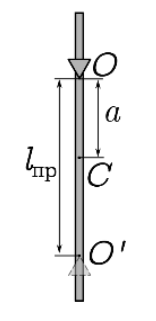
\includegraphics[width = 0.15\textwidth]{Figure 2}
    \caption{к теореме Гюйгенса}
\end{wrapfigure}

Смысл этой длины в том, что физический маятник длиной $l$, подвешенный
в точке $a$, имеет тот же период малых колебаний, что и математический
маятник длиной $l_{reduced}$.

С понятием «приведённой длины» 
\newline
связана следующая теорема (\textit{Гюйгенса}).
Рассмотрим точку $O'$, отстоящую от точки опоры $O$ на расстояние
$l_{reduced}$ вдоль стержня (эту точку иногда называют \textit{центром качания}
физического маятника). Оказывается, если маятник подвесить за точку $O'$, то
период его качания не изменится. Иными словами, точка опоры и центр качания
маятника взаимно обратимы.

\section{Экспериментальная установка}

Тонкий стальной стержень длиной $l \sim 1$ м и массой $m \sim 1$ кг (точные
параметры определяются непосредственными измерениями) подвешивается на
прикреплённой стене консоли с помощью небольшой призмы. Диаметр стержня много
меньше его длины $ d \sim 12$ мм $\ll l$. Небольшая призма крепится на стержне
винтом и острым основанием опирается на поверхность закреплённой на стене
консоли. Острие ребра призмы образует ось качания маятника. Возможны две схемы
реализации установок.

\textbf{Установка А}. Призму можно перемещать вдоль стержня, изменяя
длину $a$ — расстояние от центра масс до точки подвеса. Период колебаний
измеряется непосредственно с помощью секундомера.

\textbf{Установка Б}. Подвесная призма остаётся неподвижной $(a = const)$, а
на стержень маятника насаживается дополнительное тело небольшого размера
(«чечевица» или цилиндр), положение которого можно изменять, изменяя таким
образом момент инерции маятника. Период колебаний маятника в этой схеме
измеряется электронным счетчиком импульсов, расположенном у нижнего конца
стержня.

Расстояния во всех установках измеряются линейками и штангенциркулем.
Положение центра масс маятника может быть определено с помощью
балансирования маятника на вспомогательной T-образной подставке с
острой верхней гранью.

Измеряя зависимости периода малых колебаний от положения стержня
или дополнительного тела на нём, можно экспериментально вычислить значение
ускорения свободного падения g. Формулу (3) можно проверить, откладывая по
осям величины $u = T^2a$ и $v = a^2$ . В этих координатах график $u(v)$ должен
иметь вид прямой линии, угловой коэффициент которой пропорционален $g$, $a$
вертикальное смещение — моменту инерции стержня относительно центра масс.

\subsubsection{Измерение периода колебаний}

Мы используем электронный счётчик колебаний, поэтому случайная погрешность
крайне мала. Остаётся систематическая погрешность, равная половине последней
десятичной цифры, $\sigma_t = 0.005$ с. Также мы проводим измерения большого
количества колебаний $(n = 20)$, из-за чего погрешность одного колебания,
то есть $\sigma_T$ уменьшается в $n$ раз, то есть 
$\sigma_T = \frac{\sigma_t}{n}$.

\subsubsection{Особенности маятника с перемещаемым грузом}

Если на стержень насадить груз, то момент инерции маятника, а значит
и период его колебаний, будет зависеть от положения груза относительно
оси качания.

\begin{wrapfigure}{r}{0.40\textwidth}
    \centering
    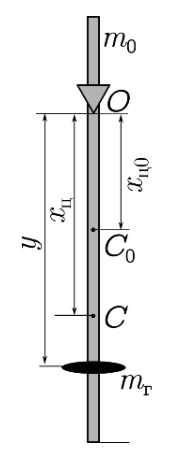
\includegraphics[width = 0.15\textwidth]{Figure 3}
    \caption{маятник с грузом}
\end{wrapfigure}

В качестве подвижного груза в работе используется металлический цилиндр или
«чечевица». Масса груза $m_g \approx 300 \div 400$ г, диаметр $d_g \sim 6$ см.
Поскольку размер груза мал по сравнению с длиной стержня, его можно
считать закреплённой на стержне точечной массой. Обозначим за $y$ расстояние
от точки подвеса $O$ до центра масс груза (см. Рис. 3). Тогда момент инерции
маятника будет равен:

\[J = J_o + m_gy^2,\]

где $J_0$ -- момент инерции маятника без груза, определяемый по формуле (1).
Поскольку точка подвеса в схеме Б фиксирована, величина $J_0$ в опыте остаётся
постоянной.

Заметим, что величину $y$ на практике измерить напрямую затруднительно,
поскольку положение центра масс груза точно не известно. Вместо этого можно
измерить положение центра масс маятника с грузом и без него.
Пусть $x_{c0}$ -- расстояние от точки подвеса (острия
призмы) до центра масс маятника без груза. Тогда центр
масс маятника с грузом находится в точке

\[x_c = \frac{m_0x_{c0} + m_gy}{M},\]

где $m_0$ - масса мятника без груза (стержня вместе с призмой),
$M = m_0 + m_g$ — полная масса маятника. Положения центра масс
$x_c$ и $x_{c0}$ могут быть измерены с помощью подставки. Отсюда находим
формулу для вычисления положения центра масс груза:

\begin{equation}
    y = \frac{Mx_c - m_0x_{c0}}{m_g}
\end{equation}

Заметим, что положение центра масс груза достаточно измерить
\newline
только один раз, а затем измерять смещение $\Delta{y}$ груза относительно
некоторого исходного положения $y_0$.

Из общей формулы (2) найдём период колебаний маятника грузом:

\begin{equation}
    T = 2\pi\sqrt{\frac{J_0 + m_gy^2}{gMx_c}}
\end{equation}

Отсюда видно, что если построить зависимость величины $u = T^2x_c$ от
$v = y^2$, то график должен иметь вид прямой линии. По её наклону можно
определить ускорение свободного падения g, а по вертикальному смещению --
момент инерции $J_0$ маятника.

\section{Задание}

\textbf{Счётчик колебаний:} $\sigma_t = 0.005$ с

\textbf{Линейка:} $\sigma_l = 0.05$ см

Погрешность $g$ зависит от точности измерения длин и периода колебаний. Длины
измеряли линейкой. Наименьшее измеренное расстояние 18 см, а наибольшее --
98 см. Абсолютная погрешность линейки: $\sigma_l = 0.05$ см.
Тогда относительная погрешность длин составляет порядка
$\varepsilon_{max} = \frac{0.05}{18} \approx 0.3\%$.

\textbf{Вывод:} используемые в работе инструменты позволяют вести измерения
длин с точностью вплоть до 0.3\%. Для получения конечного результата с данной
точностью период колебаний следует измерять с той же относительной
погрешностью: не хуже, чем $\varepsilon_{max} \approx 0.3\%$.

Далее проведём основные измерения:

\begin{center}
    \begin{tabular}{|c|c|c|}
        \hline

        & Значение & Погрешность \\
        \hline

        Длина стержня $l$, см & 98.24 & 0.05 \\

        \hline

        Длина стержня до призмы $z$, см & 71.94 & 0.05 \\

        \hline

        Положение центра масса от призмы $a$, см & 26.30 & 0.05 \\

        \hline

        Масса стержня $m$, г & 890.90 & 0.05 \\

        \hline

        Масса призмы $m_{pr}$, гр & 75.90 & 0.05 \\

        \hline

        Масса груза $m_{g}$, гр & 315.80 & 0.05 \\

        \hline

        Центр масс стержня с призмой $x_{c0}$, см & 50.04 & 0.05 \\

        \hline
    \end{tabular}
\end{center}

По формуле 1 посчитаем $J_0$, $J_0 = \frac{ml^2}{12} + ma^2 = 
\frac{0.89090 \cdot 0.9824 ^ 2}{12} + 0.89090 \cdot 0.2630^2
\approx 0.1333 kg \cdot m^2$

Теперь замерим 20 колебаний маятника без груза:

\begin{center}
    \begin{tabular}{|c|c|c|}
        \hline

        $t$, с & n & $T$, с \\

        \hline

        30.74 & 20 & 1.537 \\

        \hline
    \end{tabular}
\end{center}

из формулы (3):

\[g = \frac{4\pi^2(\frac{l^2}{12} + a^2)}{aT^2} \approx
\frac{4 \cdot 3.14^2(\frac{0.98^2}{12} + 0.26^2)}{0.26 \cdot 1.537^2}
\approx 9.49 \frac{m}{s^2}\]

Относительная погрешность $\varepsilon_g$ получилась $\approx 3\%$.

Теперь будем вешать груз на разном расстоянии от призмы и будем замерять
период колебаний.

Выведем формулу для $g$ из формулы (7):

\begin{equation}
    g = \frac{4\pi^2(J_0 + m_gy^2)}{T^2Mx_c}
\end{equation}

\begin{center}
    \begin{tabular}{|c|c|c|c|c|c|}
        \hline

        $N$ эксперимента & $t$, с & $n$ & $T$, с & $y$, см & $g, \frac{m}{s^2}$ \\
        
        \hline

        1 & 28.24 & 20.0 & 1.4120 & 26.7737 & 9.1572 \\

        \hline

        2 & 28.31 & 20.0 & 1.4155 & 29.2106 & 9.1605 \\

        \hline

        3 & 28.54 & 20.0 & 1.4270 & 34.8966 & 9.2040 \\

        \hline

        4 & 29.19 & 20.0 & 1.4595 & 43.0194 & 9.2150 \\

        \hline

        5 & 28.64 & 20.0 & 1.4320 & 12.9649 & 9.1194 \\

        \hline

        6 & 28.37 & 20.0 & 1.4185 & 16.2140 & 9.1545 \\

        \hline

        7 & 28.29 & 20.0 & 1.4145 & 23.1184 & 9.0957 \\


        \hline
    \end{tabular}
\end{center}

Построим зависимость $u(v)$, где $u = T^2x_c$,  $v = y^2$:

\newpage

\begin{figure}[h]
    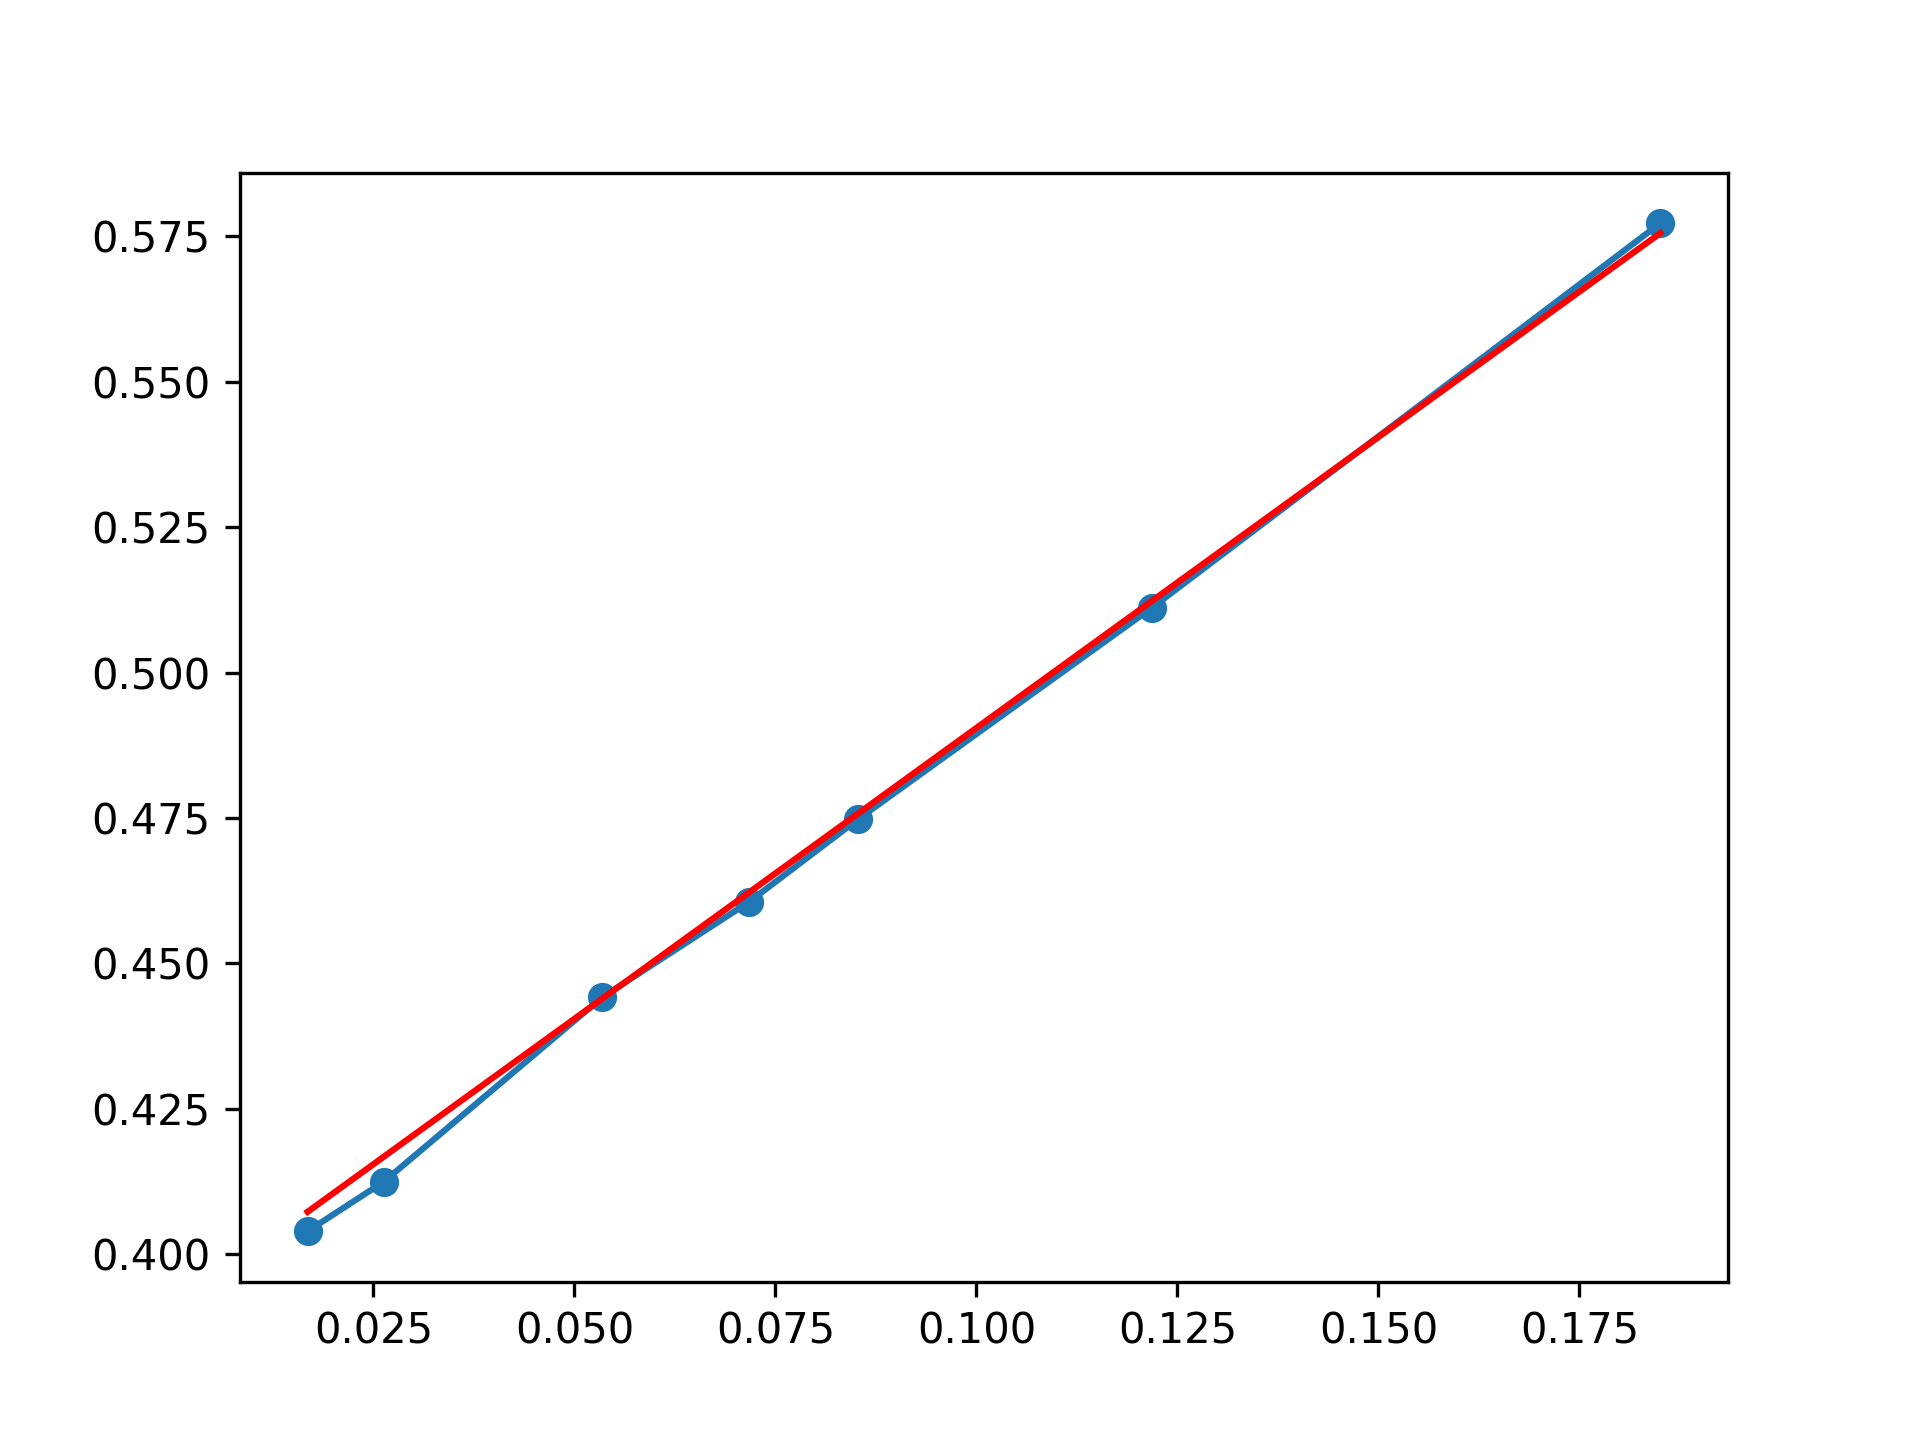
\includegraphics[width = 1\textwidth]{graph.png}
    \caption{$T^2x_c$ от $y^2$.}
\end{figure}

Из формулы (8):
\begin{equation}
    T^2x_c = \frac{4\pi^2(J_0 + m_gy^2)}{Mg} =
    \frac{4\pi^2J_0}{Mg} + \frac{4\pi^2m_gy^2}{Mg}.
\end{equation}

То есть $k$ наклона есть:
\[k = \frac{4\pi^2m_g}{Mg}.\]

Тогда:
\begin{equation}
    g = \frac{4\pi^2m_g}{Mk}.
\end{equation}

Красная линия была подобрана для лучшего совпадения с графиком. Её коэффициент
наклона $k = 1$, а значит по формуле (10) $g \approx 9.72 \frac{m}{s^2}$.

Рассчитаем погрешность $\varepsilon_g$ по табличному значению
$g_0 \approx 9.81$
тогда:
\[\varepsilon_g = (9.81 - 9.72) / (9.81) \cdot 100 \% \approx 0.92\%\]

\section{Вывод}

Метод с использованием график оказался сильно точнее (в 3 раза) чем
используя формулу и одно измерение, однако формула всё ещё довольно
хорошо описывает период колебаний маятника, так как полученный график
действительно оказался почти прямой.

\end{document}
